% Generated by Sphinx.
\def\sphinxdocclass{report}
\documentclass[letterpaper,10pt,english]{sphinxmanual}
\usepackage[utf8]{inputenc}
\DeclareUnicodeCharacter{00A0}{\nobreakspace}
\usepackage{cmap}
\usepackage[T1]{fontenc}
\usepackage{babel}
\usepackage{times}
\usepackage[Bjarne]{fncychap}
\usepackage{longtable}
\usepackage{sphinx}
\usepackage{multirow}


\title{fantastico Documentation}
\date{May 03, 2013}
\release{0.0.1-b33}
\author{Radu Viorel Cosnita}
\newcommand{\sphinxlogo}{}
\renewcommand{\releasename}{Release}
\makeindex

\makeatletter
\def\PYG@reset{\let\PYG@it=\relax \let\PYG@bf=\relax%
    \let\PYG@ul=\relax \let\PYG@tc=\relax%
    \let\PYG@bc=\relax \let\PYG@ff=\relax}
\def\PYG@tok#1{\csname PYG@tok@#1\endcsname}
\def\PYG@toks#1+{\ifx\relax#1\empty\else%
    \PYG@tok{#1}\expandafter\PYG@toks\fi}
\def\PYG@do#1{\PYG@bc{\PYG@tc{\PYG@ul{%
    \PYG@it{\PYG@bf{\PYG@ff{#1}}}}}}}
\def\PYG#1#2{\PYG@reset\PYG@toks#1+\relax+\PYG@do{#2}}

\expandafter\def\csname PYG@tok@gd\endcsname{\def\PYG@tc##1{\textcolor[rgb]{0.63,0.00,0.00}{##1}}}
\expandafter\def\csname PYG@tok@gu\endcsname{\let\PYG@bf=\textbf\def\PYG@tc##1{\textcolor[rgb]{0.50,0.00,0.50}{##1}}}
\expandafter\def\csname PYG@tok@gt\endcsname{\def\PYG@tc##1{\textcolor[rgb]{0.00,0.27,0.87}{##1}}}
\expandafter\def\csname PYG@tok@gs\endcsname{\let\PYG@bf=\textbf}
\expandafter\def\csname PYG@tok@gr\endcsname{\def\PYG@tc##1{\textcolor[rgb]{1.00,0.00,0.00}{##1}}}
\expandafter\def\csname PYG@tok@cm\endcsname{\let\PYG@it=\textit\def\PYG@tc##1{\textcolor[rgb]{0.25,0.50,0.56}{##1}}}
\expandafter\def\csname PYG@tok@vg\endcsname{\def\PYG@tc##1{\textcolor[rgb]{0.73,0.38,0.84}{##1}}}
\expandafter\def\csname PYG@tok@m\endcsname{\def\PYG@tc##1{\textcolor[rgb]{0.13,0.50,0.31}{##1}}}
\expandafter\def\csname PYG@tok@mh\endcsname{\def\PYG@tc##1{\textcolor[rgb]{0.13,0.50,0.31}{##1}}}
\expandafter\def\csname PYG@tok@cs\endcsname{\def\PYG@tc##1{\textcolor[rgb]{0.25,0.50,0.56}{##1}}\def\PYG@bc##1{\setlength{\fboxsep}{0pt}\colorbox[rgb]{1.00,0.94,0.94}{\strut ##1}}}
\expandafter\def\csname PYG@tok@ge\endcsname{\let\PYG@it=\textit}
\expandafter\def\csname PYG@tok@vc\endcsname{\def\PYG@tc##1{\textcolor[rgb]{0.73,0.38,0.84}{##1}}}
\expandafter\def\csname PYG@tok@il\endcsname{\def\PYG@tc##1{\textcolor[rgb]{0.13,0.50,0.31}{##1}}}
\expandafter\def\csname PYG@tok@go\endcsname{\def\PYG@tc##1{\textcolor[rgb]{0.20,0.20,0.20}{##1}}}
\expandafter\def\csname PYG@tok@cp\endcsname{\def\PYG@tc##1{\textcolor[rgb]{0.00,0.44,0.13}{##1}}}
\expandafter\def\csname PYG@tok@gi\endcsname{\def\PYG@tc##1{\textcolor[rgb]{0.00,0.63,0.00}{##1}}}
\expandafter\def\csname PYG@tok@gh\endcsname{\let\PYG@bf=\textbf\def\PYG@tc##1{\textcolor[rgb]{0.00,0.00,0.50}{##1}}}
\expandafter\def\csname PYG@tok@ni\endcsname{\let\PYG@bf=\textbf\def\PYG@tc##1{\textcolor[rgb]{0.84,0.33,0.22}{##1}}}
\expandafter\def\csname PYG@tok@nl\endcsname{\let\PYG@bf=\textbf\def\PYG@tc##1{\textcolor[rgb]{0.00,0.13,0.44}{##1}}}
\expandafter\def\csname PYG@tok@nn\endcsname{\let\PYG@bf=\textbf\def\PYG@tc##1{\textcolor[rgb]{0.05,0.52,0.71}{##1}}}
\expandafter\def\csname PYG@tok@no\endcsname{\def\PYG@tc##1{\textcolor[rgb]{0.38,0.68,0.84}{##1}}}
\expandafter\def\csname PYG@tok@na\endcsname{\def\PYG@tc##1{\textcolor[rgb]{0.25,0.44,0.63}{##1}}}
\expandafter\def\csname PYG@tok@nb\endcsname{\def\PYG@tc##1{\textcolor[rgb]{0.00,0.44,0.13}{##1}}}
\expandafter\def\csname PYG@tok@nc\endcsname{\let\PYG@bf=\textbf\def\PYG@tc##1{\textcolor[rgb]{0.05,0.52,0.71}{##1}}}
\expandafter\def\csname PYG@tok@nd\endcsname{\let\PYG@bf=\textbf\def\PYG@tc##1{\textcolor[rgb]{0.33,0.33,0.33}{##1}}}
\expandafter\def\csname PYG@tok@ne\endcsname{\def\PYG@tc##1{\textcolor[rgb]{0.00,0.44,0.13}{##1}}}
\expandafter\def\csname PYG@tok@nf\endcsname{\def\PYG@tc##1{\textcolor[rgb]{0.02,0.16,0.49}{##1}}}
\expandafter\def\csname PYG@tok@si\endcsname{\let\PYG@it=\textit\def\PYG@tc##1{\textcolor[rgb]{0.44,0.63,0.82}{##1}}}
\expandafter\def\csname PYG@tok@s2\endcsname{\def\PYG@tc##1{\textcolor[rgb]{0.25,0.44,0.63}{##1}}}
\expandafter\def\csname PYG@tok@vi\endcsname{\def\PYG@tc##1{\textcolor[rgb]{0.73,0.38,0.84}{##1}}}
\expandafter\def\csname PYG@tok@nt\endcsname{\let\PYG@bf=\textbf\def\PYG@tc##1{\textcolor[rgb]{0.02,0.16,0.45}{##1}}}
\expandafter\def\csname PYG@tok@nv\endcsname{\def\PYG@tc##1{\textcolor[rgb]{0.73,0.38,0.84}{##1}}}
\expandafter\def\csname PYG@tok@s1\endcsname{\def\PYG@tc##1{\textcolor[rgb]{0.25,0.44,0.63}{##1}}}
\expandafter\def\csname PYG@tok@gp\endcsname{\let\PYG@bf=\textbf\def\PYG@tc##1{\textcolor[rgb]{0.78,0.36,0.04}{##1}}}
\expandafter\def\csname PYG@tok@sh\endcsname{\def\PYG@tc##1{\textcolor[rgb]{0.25,0.44,0.63}{##1}}}
\expandafter\def\csname PYG@tok@ow\endcsname{\let\PYG@bf=\textbf\def\PYG@tc##1{\textcolor[rgb]{0.00,0.44,0.13}{##1}}}
\expandafter\def\csname PYG@tok@sx\endcsname{\def\PYG@tc##1{\textcolor[rgb]{0.78,0.36,0.04}{##1}}}
\expandafter\def\csname PYG@tok@bp\endcsname{\def\PYG@tc##1{\textcolor[rgb]{0.00,0.44,0.13}{##1}}}
\expandafter\def\csname PYG@tok@c1\endcsname{\let\PYG@it=\textit\def\PYG@tc##1{\textcolor[rgb]{0.25,0.50,0.56}{##1}}}
\expandafter\def\csname PYG@tok@kc\endcsname{\let\PYG@bf=\textbf\def\PYG@tc##1{\textcolor[rgb]{0.00,0.44,0.13}{##1}}}
\expandafter\def\csname PYG@tok@c\endcsname{\let\PYG@it=\textit\def\PYG@tc##1{\textcolor[rgb]{0.25,0.50,0.56}{##1}}}
\expandafter\def\csname PYG@tok@mf\endcsname{\def\PYG@tc##1{\textcolor[rgb]{0.13,0.50,0.31}{##1}}}
\expandafter\def\csname PYG@tok@err\endcsname{\def\PYG@bc##1{\setlength{\fboxsep}{0pt}\fcolorbox[rgb]{1.00,0.00,0.00}{1,1,1}{\strut ##1}}}
\expandafter\def\csname PYG@tok@kd\endcsname{\let\PYG@bf=\textbf\def\PYG@tc##1{\textcolor[rgb]{0.00,0.44,0.13}{##1}}}
\expandafter\def\csname PYG@tok@ss\endcsname{\def\PYG@tc##1{\textcolor[rgb]{0.32,0.47,0.09}{##1}}}
\expandafter\def\csname PYG@tok@sr\endcsname{\def\PYG@tc##1{\textcolor[rgb]{0.14,0.33,0.53}{##1}}}
\expandafter\def\csname PYG@tok@mo\endcsname{\def\PYG@tc##1{\textcolor[rgb]{0.13,0.50,0.31}{##1}}}
\expandafter\def\csname PYG@tok@mi\endcsname{\def\PYG@tc##1{\textcolor[rgb]{0.13,0.50,0.31}{##1}}}
\expandafter\def\csname PYG@tok@kn\endcsname{\let\PYG@bf=\textbf\def\PYG@tc##1{\textcolor[rgb]{0.00,0.44,0.13}{##1}}}
\expandafter\def\csname PYG@tok@o\endcsname{\def\PYG@tc##1{\textcolor[rgb]{0.40,0.40,0.40}{##1}}}
\expandafter\def\csname PYG@tok@kr\endcsname{\let\PYG@bf=\textbf\def\PYG@tc##1{\textcolor[rgb]{0.00,0.44,0.13}{##1}}}
\expandafter\def\csname PYG@tok@s\endcsname{\def\PYG@tc##1{\textcolor[rgb]{0.25,0.44,0.63}{##1}}}
\expandafter\def\csname PYG@tok@kp\endcsname{\def\PYG@tc##1{\textcolor[rgb]{0.00,0.44,0.13}{##1}}}
\expandafter\def\csname PYG@tok@w\endcsname{\def\PYG@tc##1{\textcolor[rgb]{0.73,0.73,0.73}{##1}}}
\expandafter\def\csname PYG@tok@kt\endcsname{\def\PYG@tc##1{\textcolor[rgb]{0.56,0.13,0.00}{##1}}}
\expandafter\def\csname PYG@tok@sc\endcsname{\def\PYG@tc##1{\textcolor[rgb]{0.25,0.44,0.63}{##1}}}
\expandafter\def\csname PYG@tok@sb\endcsname{\def\PYG@tc##1{\textcolor[rgb]{0.25,0.44,0.63}{##1}}}
\expandafter\def\csname PYG@tok@k\endcsname{\let\PYG@bf=\textbf\def\PYG@tc##1{\textcolor[rgb]{0.00,0.44,0.13}{##1}}}
\expandafter\def\csname PYG@tok@se\endcsname{\let\PYG@bf=\textbf\def\PYG@tc##1{\textcolor[rgb]{0.25,0.44,0.63}{##1}}}
\expandafter\def\csname PYG@tok@sd\endcsname{\let\PYG@it=\textit\def\PYG@tc##1{\textcolor[rgb]{0.25,0.44,0.63}{##1}}}

\def\PYGZbs{\char`\\}
\def\PYGZus{\char`\_}
\def\PYGZob{\char`\{}
\def\PYGZcb{\char`\}}
\def\PYGZca{\char`\^}
\def\PYGZam{\char`\&}
\def\PYGZlt{\char`\<}
\def\PYGZgt{\char`\>}
\def\PYGZsh{\char`\#}
\def\PYGZpc{\char`\%}
\def\PYGZdl{\char`\$}
\def\PYGZhy{\char`\-}
\def\PYGZsq{\char`\'}
\def\PYGZdq{\char`\"}
\def\PYGZti{\char`\~}
% for compatibility with earlier versions
\def\PYGZat{@}
\def\PYGZlb{[}
\def\PYGZrb{]}
\makeatother

\begin{document}

\maketitle
\tableofcontents
\phantomsection\label{index::doc}



\chapter{Introduction}
\label{intro:introduction}\label{intro::doc}\label{intro:fantastico-framework}

\section{Why another python framework?}
\label{intro:why-another-python-framework}
The main reason for developing a new framework is simple: I want to use it for teaching purposes. I have seen
many projects which fail either because of poor coding or because they become legacy very fast. I will not get into details
why and what could have been done. It defeats the purpose.

Each piece of code that is being added to fantastico will follow these simple rules:
\begin{enumerate}
\item {} 
\emph{The code is written because is needed and there is no clean way to achieve the requirement with existing fantastico features}.

\item {} 
The code is developed using TDD (Test Driven Development).

\item {} 
The code quality is 9+ (reported by pylint).

\item {} 
The code coverage is 90\%+ (reported by nose coverage).

\item {} 
The code is fully documented and included into documentation.

\end{enumerate}


\subsection{What do you want to teach who?}
\label{intro:what-do-you-want-to-teach-who}
I am a big fan of Agile practices and currently I own a domain called scrum-expert.ro. This is meant to become a collection of
hands on resource of how to develop good software with high quality and in a reasonable amount of time. Resources will cover topics
like
\begin{enumerate}
\item {} 
Incremental development always ready for rollout.

\item {} 
TDD (Test Driven Development)

\item {} 
XP (eXtreme programming)

\item {} 
Scrum

\item {} 
Projects setup for Continuous Delivery

\end{enumerate}

and many other topics that are required for delivering high quality software but apparently so many companies are ignoring nowadays.


\section{Fantastico's initial ideas}
\label{intro:fantastico-s-initial-ideas}\begin{itemize}
\item {} 
Very fast and pluggable routing engine.

\item {} 
Easily creation of REST apis.

\item {} 
Easily publishing of content (dynamic content).

\item {} 
Easily composition of available content.

\item {} 
Easily deployment on non expensive infrastructures (AWS, RackSpace).

\end{itemize}

Once the features above are developed there should be extremely easy to create the following sample applications:
\begin{enumerate}
\item {} 
Blog development

\item {} 
Web Forms development.

\item {} 
Personal web sites.

\end{enumerate}


\chapter{Getting started}
\label{get_started/getting_started:getting-started}\label{get_started/getting_started::doc}

\section{Installation manual}
\label{get_started/installation:installation-manual}\label{get_started/installation::doc}
In this section you can find out how to configure fantastico framework for different purposes.


\subsection{Developing a new fantastico project}
\label{get_started/installation:developing-a-new-fantastico-project}
Currently fantastico is in early stages so we did not really use it to create new projects. The desired way we want
to provide this is presented below:

pip-3.2 install fantastico

Done, now you are ready to follow our tutorials about creating new projects.


\subsection{Contributing to fantastico framework}
\label{get_started/installation:contributing-to-fantastico-framework}
Fantastico is an open source MIT licensed project to which any contribution is welcomed. If you like this framework idea
and you want to contribute do the following (I assume you are on an ubuntu machine):

\begin{Verbatim}[commandchars=\\\{\}]
\PYG{c}{\PYGZsh{}. Create a github account.}
\PYG{c}{\PYGZsh{}. Ask for permissions to contribute to this project (send an email to radu.cosnita@gmail.com) \PYGZhy{} I will gladly grant you permissions.}
\PYG{c}{\PYGZsh{}. Create a folder where you want to hold fantastico framework files. (e.g worspace\PYGZus{}fantastico)}
\PYG{c}{\PYGZsh{}. cd \PYGZti{}/workspace\PYGZus{}fantastico}
\PYG{c}{\PYGZsh{}. git clone git@github.com:rcosnita/fantastico}
\PYG{c}{\PYGZsh{}. sudo apt\PYGZhy{}get install python3\PYGZhy{}setuptools}
\PYG{c}{\PYGZsh{}. sh virtual\PYGZus{}env/setup\PYGZus{}dev\PYGZus{}env.sh}
\PYG{c}{\PYGZsh{}. cd \PYGZti{}/workspace\PYGZus{}fantastico}
\PYG{c}{\PYGZsh{}. git clone git@github.com:rcosnita/fantastico fantastico\PYGZhy{}doc}
\PYG{c}{\PYGZsh{}. git checkout gh\PYGZhy{}pages}
\end{Verbatim}

Now you have a fully functional fantastico workspace. I personally use PyDev and spring toolsuite but you are free to use
whatever editor you want. The only rule we follow is \emph{always keep the code stable}. To check the stability of your contribution
before commiting the code follow the steps below:

\begin{Verbatim}[commandchars=\\\{\}]
\PYG{c}{\PYGZsh{}. cd \PYGZti{}/workspace\PYGZus{}fantastico/fantastico/fantastico}
\PYG{c}{\PYGZsh{}. sh run\PYGZus{}tests.sh (we expect no failure in here)}
\PYG{c}{\PYGZsh{}. sh run\PYGZus{}pylint.sh (we expect 9+ rated code otherwise the build will fail).}
\PYG{c}{\PYGZsh{}. cd \PYGZti{}/workspace\PYGZus{}fantastico/fantastico}
\PYG{c}{\PYGZsh{}. export BUILD\PYGZus{}NUMBER=1}
\PYG{c}{\PYGZsh{}. ./build\PYGZus{}docs.sh (this will autogenerate documentation).}
\PYG{c}{\PYGZsh{}. Look into \PYGZti{}/workspace\PYGZus{}fantastico/fantastico\PYGZhy{}doc}
\PYG{c}{\PYGZsh{}. Here you can see the autogenerated documentation (do not commit this as Jenkins will do this for you).}
\PYG{c}{\PYGZsh{}. Be brave and push your newly awesome contribution.}
\end{Verbatim}


\section{Fantastico settings}
\label{get_started/settings:fantastico-settings}\label{get_started/settings::doc}
Fantastico is configured using a plain settings file. This file is located in the root of fantastico framework or in the root
folder of your project. Before we dig further into configuration options lets see a very simple settings file:

\begin{Verbatim}[commandchars=\\\{\}]
\PYG{k}{class} \PYG{n+nc}{BasicSettings}\PYG{p}{(}\PYG{n+nb}{object}\PYG{p}{)}\PYG{p}{:}
   \PYG{n+nd}{@property}
   \PYG{k}{def} \PYG{n+nf}{installed\PYGZus{}middleware}\PYG{p}{(}\PYG{n+nb+bp}{self}\PYG{p}{)}\PYG{p}{:}
      \PYG{k}{return} \PYG{p}{[}\PYG{l+s}{\PYGZdq{}}\PYG{l+s}{fantastico.middleware.request\PYGZus{}middleware.RequestMiddleware}\PYG{l+s}{\PYGZdq{}}\PYG{p}{,}
             \PYG{l+s}{\PYGZdq{}}\PYG{l+s}{fantastico.middleware.routing\PYGZus{}middleware.RoutingMiddleware}\PYG{l+s}{\PYGZdq{}}\PYG{p}{]}

   \PYG{n+nd}{@property}
   \PYG{k}{def} \PYG{n+nf}{supported\PYGZus{}languages}\PYG{p}{(}\PYG{n+nb+bp}{self}\PYG{p}{)}\PYG{p}{:}
      \PYG{k}{return} \PYG{p}{[}\PYG{l+s}{\PYGZdq{}}\PYG{l+s}{en\PYGZus{}us}\PYG{l+s}{\PYGZdq{}}\PYG{p}{]}
\end{Verbatim}

The above code sample represent the minimum required configuration for fantastico framework to run. The order in which middlewares
are listed is the order in which they are executed when an http request is made.


\subsection{Settings API}
\label{get_started/settings:settings-api}
Below you can find technical information about settings.
\index{BasicSettings (class in fantastico.settings)}

\begin{fulllineitems}
\phantomsection\label{get_started/settings:fantastico.settings.BasicSettings}\pysigline{\strong{class }\code{fantastico.settings.}\bfcode{BasicSettings}}
This is the core class that describes all available settings of fantastico framework. For convenience all options
have default values that ensure minimum functionality of the framework. Below you can find an example of three possible 
configuration: Dev / Stage / Production.

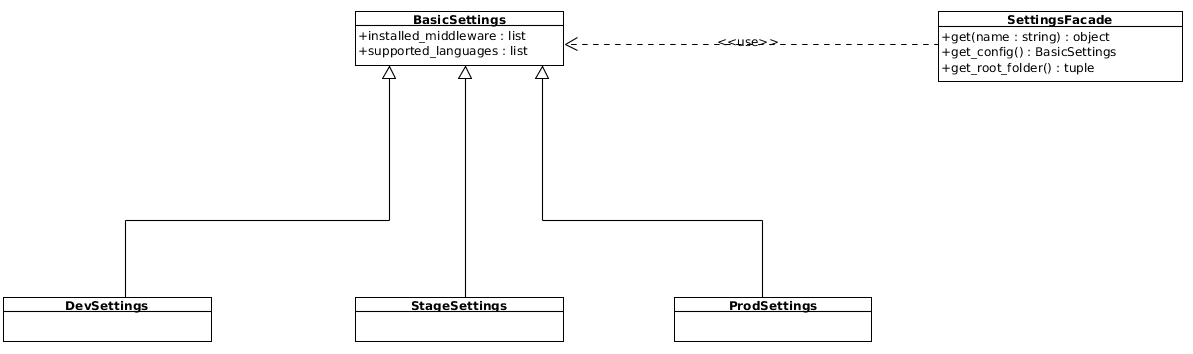
\includegraphics{settings.png}

As you can see, if you want to overwrite basic configuration you simply have to extend the class and set new values
for the attributes you want to overwrite.
\index{installed\_middleware (fantastico.settings.BasicSettings attribute)}

\begin{fulllineitems}
\phantomsection\label{get_started/settings:fantastico.settings.BasicSettings.installed_middleware}\pysigline{\bfcode{installed\_middleware}}
Property that holds all installed middlewares.

\end{fulllineitems}

\index{routes\_loaders (fantastico.settings.BasicSettings attribute)}

\begin{fulllineitems}
\phantomsection\label{get_started/settings:fantastico.settings.BasicSettings.routes_loaders}\pysigline{\bfcode{routes\_loaders}}
This property holds all routes loaders available.

\end{fulllineitems}

\index{supported\_languages (fantastico.settings.BasicSettings attribute)}

\begin{fulllineitems}
\phantomsection\label{get_started/settings:fantastico.settings.BasicSettings.supported_languages}\pysigline{\bfcode{supported\_languages}}
Property that holds all supported languages by this fantastico instance.

\end{fulllineitems}


\end{fulllineitems}



\subsection{Create Dev configuration}
\label{get_started/settings:create-dev-configuration}
Let's imagine you want to create a custom dev configuration for your project. Below you can find the code for this:

\begin{Verbatim}[commandchars=\\\{\}]
\PYG{k}{class} \PYG{n+nc}{DevSettings}\PYG{p}{(}\PYG{n}{BasicSettings}\PYG{p}{)}\PYG{p}{:}
   \PYG{n+nd}{@property}
   \PYG{k}{def} \PYG{n+nf}{supported\PYGZus{}languages}\PYG{p}{(}\PYG{n+nb+bp}{self}\PYG{p}{)}\PYG{p}{:}
      \PYG{k}{return} \PYG{p}{[}\PYG{l+s}{\PYGZdq{}}\PYG{l+s}{en\PYGZus{}us}\PYG{l+s}{\PYGZdq{}}\PYG{p}{,} \PYG{l+s}{\PYGZdq{}}\PYG{l+s}{ro\PYGZus{}ro}\PYG{l+s}{\PYGZdq{}}\PYG{p}{]}
\end{Verbatim}

The above configuration actually overwrites supported languages. This mean that only en\_us is relevant for \textbf{Dev} environment.
You can do the same for \textbf{Stage}, \textbf{Prod} or any other custom configuration.


\subsection{Using a specifc configuration}
\label{get_started/settings:using-a-specifc-configuration}\index{SettingsFacade (class in fantastico.settings)}

\begin{fulllineitems}
\phantomsection\label{get_started/settings:fantastico.settings.SettingsFacade}\pysiglinewithargsret{\strong{class }\code{fantastico.settings.}\bfcode{SettingsFacade}}{\emph{environ=None}}{}
For using a specific fantastico configuration you need to do two simple steps:
\begin{itemize}
\item {} 
Set \textbf{FANTASTICO\_ACTIVE\_CONFIG} environment variable to the fully python qualified class name you want to use. E.g: {\hyperref[get_started/settings:fantastico.settings.BasicSettings]{\code{fantastico.settings.BasicSettings}}}

\item {} 
In your code, you can use the following snippet to access a specific setting:

\begin{Verbatim}[commandchars=\\\{\}]
\PYG{k+kn}{from} \PYG{n+nn}{fantastico.settings} \PYG{k+kn}{import} \PYG{n}{SettingsFacade}

\PYG{k}{print}\PYG{p}{(}\PYG{n}{SettingsFacade}\PYG{p}{(}\PYG{p}{)}\PYG{o}{.}\PYG{n}{get}\PYG{p}{(}\PYG{l+s}{\PYGZdq{}}\PYG{l+s}{installed\PYGZus{}middleware}\PYG{l+s}{\PYGZdq{}}\PYG{p}{)}\PYG{p}{)}
\end{Verbatim}

\end{itemize}

If no active configuration is set in the {\hyperref[get_started/settings:fantastico.settings.BasicSettings]{\code{fantastico.settings.BasicSettings}}} will be used.
\index{get() (fantastico.settings.SettingsFacade method)}

\begin{fulllineitems}
\phantomsection\label{get_started/settings:fantastico.settings.SettingsFacade.get}\pysiglinewithargsret{\bfcode{get}}{\emph{name}}{}
Method used to retrieve a setting value.
\begin{quote}\begin{description}
\item[{Parameters}] \leavevmode\begin{itemize}
\item {} 
\textbf{name} -- Setting name.

\item {} 
\textbf{type} -- string

\end{itemize}

\item[{Returns}] \leavevmode
The setting value.

\item[{Return type}] \leavevmode
object

\end{description}\end{quote}

\end{fulllineitems}

\index{get\_config() (fantastico.settings.SettingsFacade method)}

\begin{fulllineitems}
\phantomsection\label{get_started/settings:fantastico.settings.SettingsFacade.get_config}\pysiglinewithargsret{\bfcode{get\_config}}{}{}
Method used to return the active configuration which is used by this facade.
\begin{quote}\begin{description}
\item[{Return type}] \leavevmode
{\hyperref[get_started/settings:fantastico.settings.BasicSettings]{\code{fantastico.settings.BasicSettings}}}

\item[{Returns}] \leavevmode
Active configuration currently used.

\end{description}\end{quote}

\end{fulllineitems}


\end{fulllineitems}



\section{Contribute}
\label{get_started/contribute:contribute}\label{get_started/contribute::doc}
Fantastico framework is open source so every contribution is welcome. For the moment we are looking for more developers willing to
contribute.


\subsection{Code contribution}
\label{get_started/contribute:code-contribution}
If you want to contribute with code to fantastico framework there are a simple set of rules that you must follow:
\begin{itemize}
\item {} 
Write unit tests (for the code / feature you are contributing).

\item {} 
Write integration tests (for the code / feature you are contributing).

\item {} 
Make sure your code is rated above 9.5 by pylint tool.

\item {} 
In addition integration tests and unit tests must cover 95\% of your code.

\end{itemize}

In order for each build to remain stable the following hard limits are imposed:
\begin{enumerate}
\item {} 
Unit tests must cover \textgreater{}= 95\% of the code.

\item {} 
Integration tests must cover \textgreater{}= 95\% of the code.

\item {} 
Code must be rated above 9.5 by pylint.

\item {} 
Everything must pass.

\end{enumerate}

When you push on master a set of jobs are cascaded executed:
\begin{enumerate}
\item {} 
Run all unit tests job.

\item {} 
Run all integration tests job (only if unit tests succeeds).

\item {} 
Generate documentation and publish it (only if integration tests job succeeds).

\end{enumerate}

You can follow the above build process by visiting
\href{http://jenkins.scrum-expert.ro:8080/job/fantastico-framework/}{Jenkins build}. Login with your github account and everything
should work smoothly.

In the end do not forget that in Fantastico framework we love to develop against a \textbf{stable} base. We really think code will have
high quality and zero bugs.


\subsubsection{Writing unit tests}
\label{get_started/contribute:writing-unit-tests}
For better understanding how to write unit tests see the documentation below:
\index{FantasticoUnitTestsCase (class in fantastico.tests.base\_case)}

\begin{fulllineitems}
\phantomsection\label{get_started/contribute:fantastico.tests.base_case.FantasticoUnitTestsCase}\pysiglinewithargsret{\strong{class }\code{fantastico.tests.base\_case.}\bfcode{FantasticoUnitTestsCase}}{\emph{methodName='runTest'}}{}
This is the base class that must be inherited by each unit test written for fantastico.

\begin{Verbatim}[commandchars=\\\{\}]
\PYG{k}{class} \PYG{n+nc}{SimpleUnitTest}\PYG{p}{(}\PYG{n}{FantasticoUnitTestsCase}\PYG{p}{)}\PYG{p}{:}
    \PYG{k}{def} \PYG{n+nf}{init}\PYG{p}{(}\PYG{n+nb+bp}{self}\PYG{p}{)}\PYG{p}{:}
        \PYG{n+nb+bp}{self}\PYG{o}{.}\PYG{n}{\PYGZus{}msg} \PYG{o}{=} \PYG{l+s}{\PYGZdq{}}\PYG{l+s}{Hello world}\PYG{l+s}{\PYGZdq{}}
        
    \PYG{k}{def} \PYG{n+nf}{test\PYGZus{}simple\PYGZus{}flow\PYGZus{}ok}\PYG{p}{(}\PYG{n+nb+bp}{self}\PYG{p}{)}\PYG{p}{:}
        \PYG{n+nb+bp}{self}\PYG{o}{.}\PYG{n}{assertEqual}\PYG{p}{(}\PYG{l+s}{\PYGZdq{}}\PYG{l+s}{Hello world}\PYG{l+s}{\PYGZdq{}}\PYG{p}{,} \PYG{n+nb+bp}{self}\PYG{o}{.}\PYG{n}{\PYGZus{}msg}\PYG{p}{)}
\end{Verbatim}

\end{fulllineitems}



\subsubsection{Writing integration tests}
\label{get_started/contribute:writing-integration-tests}
For better understanding how to write integration tests see the documentation below:
\index{FantasticoIntegrationTestCase (class in fantastico.tests.base\_case)}

\begin{fulllineitems}
\phantomsection\label{get_started/contribute:fantastico.tests.base_case.FantasticoIntegrationTestCase}\pysiglinewithargsret{\strong{class }\code{fantastico.tests.base\_case.}\bfcode{FantasticoIntegrationTestCase}}{\emph{methodName='runTest'}}{}
This is the base class that must be inherited by each integration test written for fantastico.

\begin{Verbatim}[commandchars=\\\{\}]
\PYG{k}{class} \PYG{n+nc}{SimpleIntegration}\PYG{p}{(}\PYG{n}{FantasticoIntegrationTestCase}\PYG{p}{)}\PYG{p}{:}
    \PYG{k}{def} \PYG{n+nf}{init}\PYG{p}{(}\PYG{n+nb+bp}{self}\PYG{p}{)}\PYG{p}{:}
        \PYG{n+nb+bp}{self}\PYG{o}{.}\PYG{n}{simple\PYGZus{}class} \PYG{o}{=} \PYG{p}{\PYGZob{}}\PYG{p}{\PYGZcb{}}
    
    \PYG{k}{def} \PYG{n+nf}{cleanup}\PYG{p}{(}\PYG{n+nb+bp}{self}\PYG{p}{)}\PYG{p}{:}
        \PYG{n+nb+bp}{self}\PYG{o}{.}\PYG{n}{simple\PYGZus{}class} \PYG{o}{=} \PYG{n+nb+bp}{None}
    
    \PYG{k}{def} \PYG{n+nf}{test\PYGZus{}simple\PYGZus{}ok}\PYG{p}{(}\PYG{n+nb+bp}{self}\PYG{p}{)}\PYG{p}{:}
        \PYG{k}{def} \PYG{n+nf}{do\PYGZus{}stuff}\PYG{p}{(}\PYG{n}{env}\PYG{p}{,} \PYG{n}{env\PYGZus{}cls}\PYG{p}{)}\PYG{p}{:}
            \PYG{n+nb+bp}{self}\PYG{o}{.}\PYG{n}{assertEqual}\PYG{p}{(}\PYG{n}{simple\PYGZus{}class}\PYG{p}{[}\PYG{n}{env}\PYG{p}{]}\PYG{p}{,} \PYG{n}{env\PYGZus{}cls}\PYG{p}{)}
            
        \PYG{n+nb+bp}{self}\PYG{o}{.}\PYG{n}{\PYGZus{}run\PYGZus{}test\PYGZus{}all\PYGZus{}envs}\PYG{p}{(}\PYG{n}{do\PYGZus{}stuff}\PYG{p}{)}
\end{Verbatim}

If you used this class you don't have to mind about restoring call methods from each middleware once they are wrapped
by fantastico app. This is a must because otherwise you will crash other tests.
\index{\_envs (fantastico.tests.base\_case.FantasticoIntegrationTestCase attribute)}

\begin{fulllineitems}
\phantomsection\label{get_started/contribute:fantastico.tests.base_case.FantasticoIntegrationTestCase._envs}\pysigline{\bfcode{\_envs}}
Private property that holds the environments against which we run the integration tests.

\end{fulllineitems}

\index{\_restore\_call\_methods() (fantastico.tests.base\_case.FantasticoIntegrationTestCase method)}

\begin{fulllineitems}
\phantomsection\label{get_started/contribute:fantastico.tests.base_case.FantasticoIntegrationTestCase._restore_call_methods}\pysiglinewithargsret{\bfcode{\_restore\_call\_methods}}{}{}
This method restore original call methods to all affected middlewares.

\end{fulllineitems}

\index{\_run\_test\_all\_envs() (fantastico.tests.base\_case.FantasticoIntegrationTestCase method)}

\begin{fulllineitems}
\phantomsection\label{get_started/contribute:fantastico.tests.base_case.FantasticoIntegrationTestCase._run_test_all_envs}\pysiglinewithargsret{\bfcode{\_run\_test\_all\_envs}}{\emph{callable\_obj}}{}
This method is used to execute a callable block of code on all environments. This is extremely useful for
avoid boiler plate code duplication and executing test logic against all environments.

\end{fulllineitems}

\index{\_save\_call\_methods() (fantastico.tests.base\_case.FantasticoIntegrationTestCase method)}

\begin{fulllineitems}
\phantomsection\label{get_started/contribute:fantastico.tests.base_case.FantasticoIntegrationTestCase._save_call_methods}\pysiglinewithargsret{\bfcode{\_save\_call\_methods}}{\emph{middlewares}}{}
This method save all call methods for each listed middleware so that later on they can be restored.

\end{fulllineitems}


\end{fulllineitems}



\chapter{Fantastico features}
\label{features/features::doc}\label{features/features:fantastico-features}

\section{Exceptions hierarchy}
\label{features/exceptions:exceptions-hierarchy}\label{features/exceptions::doc}\index{FantasticoError (class in fantastico.exceptions)}

\begin{fulllineitems}
\phantomsection\label{features/exceptions:fantastico.exceptions.FantasticoError}\pysigline{\strong{class }\code{fantastico.exceptions.}\bfcode{FantasticoError}}~
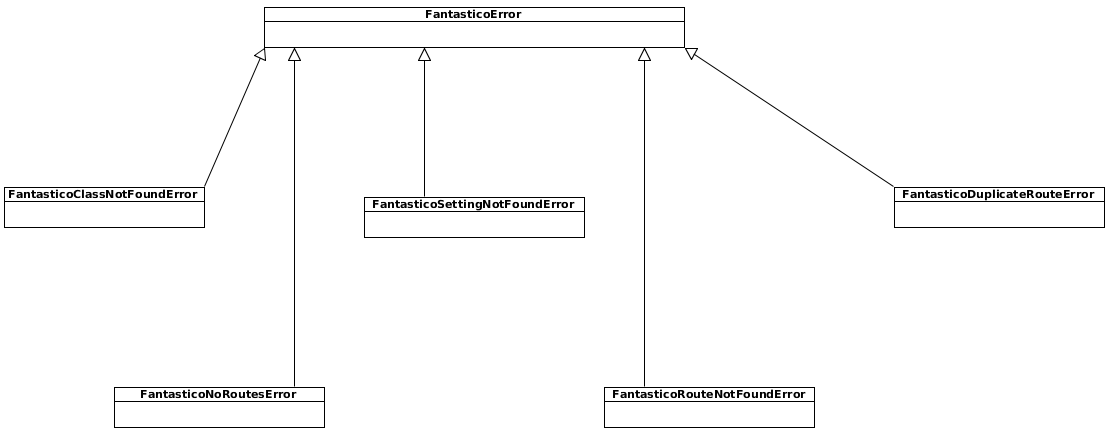
\includegraphics{exceptions.png}

\textbf{FantasticoError} is the base of all exceptions raised within fantastico framework. It describe common attributes that
each concrete fantastico exception must provide. By default all fantastico exceptions inherit FantasticoError exception. 
We do this because each raised unhandled FantasticoError is map to a specific exception response. This strategy guarantees
that at no moment errors will cause fantastico framework wsgi container to crash.

\end{fulllineitems}

\index{FantasticoClassNotFoundError (class in fantastico.exceptions)}

\begin{fulllineitems}
\phantomsection\label{features/exceptions:fantastico.exceptions.FantasticoClassNotFoundError}\pysigline{\strong{class }\code{fantastico.exceptions.}\bfcode{FantasticoClassNotFoundError}}
This exception is raised whenever code tries to dynamically import and instantiate a class which can not be resolved.

\end{fulllineitems}

\index{FantasticoSettingNotFoundError (class in fantastico.exceptions)}

\begin{fulllineitems}
\phantomsection\label{features/exceptions:fantastico.exceptions.FantasticoSettingNotFoundError}\pysigline{\strong{class }\code{fantastico.exceptions.}\bfcode{FantasticoSettingNotFoundError}}
This exception is raised whenever code tries to obtain a setting that is not available in the current fantastico
configuration.

\end{fulllineitems}

\index{FantasticoDuplicateRouteError (class in fantastico.exceptions)}

\begin{fulllineitems}
\phantomsection\label{features/exceptions:fantastico.exceptions.FantasticoDuplicateRouteError}\pysigline{\strong{class }\code{fantastico.exceptions.}\bfcode{FantasticoDuplicateRouteError}}
This exception is usually raised by routing engine when it detects duplicate routes.

\end{fulllineitems}

\index{FantasticoNoRoutesError (class in fantastico.exceptions)}

\begin{fulllineitems}
\phantomsection\label{features/exceptions:fantastico.exceptions.FantasticoNoRoutesError}\pysigline{\strong{class }\code{fantastico.exceptions.}\bfcode{FantasticoNoRoutesError}}
This exception is usually raised by routing engine when no loaders are configured or no routes are registered.

\end{fulllineitems}

\index{FantasticoRouteNotFoundError (class in fantastico.exceptions)}

\begin{fulllineitems}
\phantomsection\label{features/exceptions:fantastico.exceptions.FantasticoRouteNotFoundError}\pysigline{\strong{class }\code{fantastico.exceptions.}\bfcode{FantasticoRouteNotFoundError}}
This exception is usually raised by routing engine when a requested url is not registered.

\end{fulllineitems}

\index{FantasticoNoRequestError (class in fantastico.exceptions)}

\begin{fulllineitems}
\phantomsection\label{features/exceptions:fantastico.exceptions.FantasticoNoRequestError}\pysigline{\strong{class }\code{fantastico.exceptions.}\bfcode{FantasticoNoRequestError}}
This exception is usually raised when some components try to use fantastico.request from WSGI environ before 
{\hyperref[features/request_response:fantastico.middleware.request_middleware.RequestMiddleware]{\code{fantastico.middleware.request\_middleware.RequestMiddleware}}} was executed.

\end{fulllineitems}

\index{FantasticoContentTypeError (class in fantastico.exceptions)}

\begin{fulllineitems}
\phantomsection\label{features/exceptions:fantastico.exceptions.FantasticoContentTypeError}\pysigline{\strong{class }\code{fantastico.exceptions.}\bfcode{FantasticoContentTypeError}}
This exception is usually thrown when a mismatch between request content type and received content type differ. In
Fantastico we think it's mandatory to fulfill requests correctly and to take in consideration sent headers.

\end{fulllineitems}



\section{Request lifecycle}
\label{features/request_response:request-lifecycle}\label{features/request_response::doc}
In this document you can find how a request is processed by fantastico framework. By default WSGI applications use a dictionary
that contains various useful keys:
\begin{itemize}
\item {} 
HTTP Headers

\item {} 
HTTP Cookies

\item {} 
Helper keys (e.g file wrapper).

\end{itemize}

In fantastico we want to hide the complexity of this dictionary and allow developers to use some standardized objects. Fantastico
framework follows a Request / Response paradigm. This mean that for every single http request only one single http response will
be generated. Below, you can find a simple example of how requests are processed by fantastico framework:

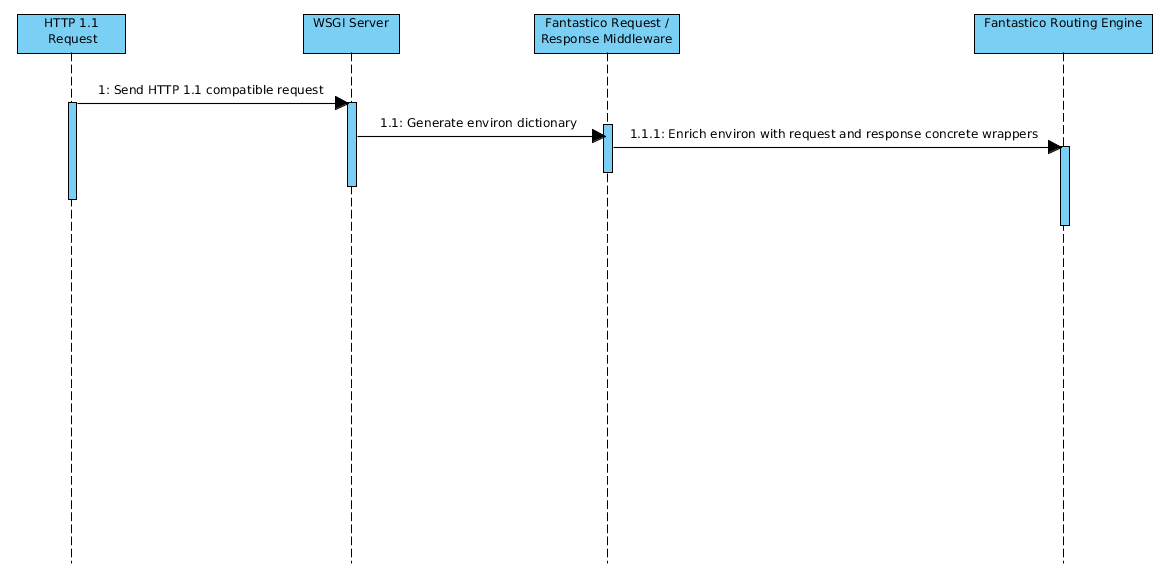
\includegraphics{request_response_sd.png}

In order to not reinvent the wheels fantastico relies on WebOb python framework in order to correctly generate request and
response objects. For more information read \href{http://docs.webob.org/en/latest/reference.html}{WebOB Doc}.


\subsection{Request middleware}
\label{features/request_response:request-middleware}
To have very good control of how WSGI environ is wrapped into \textbf{WebOb request} object a middleware component is configured. This
is the first middleware that is executed for every single http request.
\index{RequestMiddleware (class in fantastico.middleware.request\_middleware)}

\begin{fulllineitems}
\phantomsection\label{features/request_response:fantastico.middleware.request_middleware.RequestMiddleware}\pysiglinewithargsret{\strong{class }\code{fantastico.middleware.request\_middleware.}\bfcode{RequestMiddleware}}{\emph{app}}{}
This class provides the middleware responsible for converting wsgi environ dictionary into a request. The result is saved
into current WSGI environ under key \textbf{fantastico.request}.

\end{fulllineitems}



\subsection{Request context}
\label{features/request_response:request-context}
In comparison with WebOb \textbf{Fantastico} provides a nice improvement. For facilitating easy development of code, each fantastico
request has a special attribute called context. Below you can find the attributes of a request context object:
\begin{itemize}
\item {} 
settings facade ({\hyperref[get_started/settings::doc]{\emph{Fantastico settings}}})

\item {} 
session (not yet supported)

\item {} 
\textbf{language} The current preferred by user. This is determined based on user lang header.

\item {} 
user (not yet supported)

\end{itemize}
\index{RequestContext (class in fantastico.middleware.request\_context)}

\begin{fulllineitems}
\phantomsection\label{features/request_response:fantastico.middleware.request_context.RequestContext}\pysiglinewithargsret{\strong{class }\code{fantastico.middleware.request\_context.}\bfcode{RequestContext}}{\emph{settings}, \emph{language}}{}
This class holds various attributes useful giving a context to an http request. Among other things we need 
to be able to access current language, current session and possible current user profile.
\index{language (fantastico.middleware.request\_context.RequestContext attribute)}

\begin{fulllineitems}
\phantomsection\label{features/request_response:fantastico.middleware.request_context.RequestContext.language}\pysigline{\bfcode{language}}
Property that holds the current language that must be used during this request.

\end{fulllineitems}

\index{settings (fantastico.middleware.request\_context.RequestContext attribute)}

\begin{fulllineitems}
\phantomsection\label{features/request_response:fantastico.middleware.request_context.RequestContext.settings}\pysigline{\bfcode{settings}}
Property that holds the current settings facade used for accessing fantastico configuration.

\end{fulllineitems}


\end{fulllineitems}



\subsection{Obtain request language}
\label{features/request_response:obtain-request-language}\index{Language (class in fantastico.locale.language)}

\begin{fulllineitems}
\phantomsection\label{features/request_response:fantastico.locale.language.Language}\pysiglinewithargsret{\strong{class }\code{fantastico.locale.language.}\bfcode{Language}}{\emph{code}}{}
Class used to define how does language object looks like. There are various use cases for using language but
the simplest one is in request context object:

\begin{Verbatim}[commandchars=\\\{\}]
\PYG{n}{language} \PYG{o}{=} \PYG{n}{request}\PYG{o}{.}\PYG{n}{context}\PYG{o}{.}\PYG{n}{language}

\PYG{k}{if} \PYG{n}{language}\PYG{o}{.}\PYG{n}{code} \PYG{o}{=} \PYG{l+s}{\PYGZdq{}}\PYG{l+s}{en\PYGZus{}us}\PYG{l+s}{\PYGZdq{}}\PYG{p}{:}
   \PYG{k}{print}\PYG{p}{(}\PYG{l+s}{\PYGZdq{}}\PYG{l+s}{English (US) language}\PYG{l+s}{\PYGZdq{}}\PYG{p}{)}\PYG{o}{.}
\PYG{k}{else}\PYG{p}{:}
   \PYG{k}{raise} \PYG{n+ne}{Exception}\PYG{p}{(}\PYG{l+s}{\PYGZdq{}}\PYG{l+s}{Language }\PYG{l+s+si}{\PYGZpc{}s}\PYG{l+s}{ is not supported.}\PYG{l+s}{\PYGZdq{}} \PYG{o}{\PYGZpc{}} \PYG{n}{language}\PYG{o}{.}\PYG{n}{code}\PYG{p}{)}
\end{Verbatim}
\index{code (fantastico.locale.language.Language attribute)}

\begin{fulllineitems}
\phantomsection\label{features/request_response:fantastico.locale.language.Language.code}\pysigline{\bfcode{code}}
Property that holds the language code. This is readonly because once instantiated we mustn't be able to change it.

\end{fulllineitems}


\end{fulllineitems}



\subsection{Obtain settings using request}
\label{features/request_response:obtain-settings-using-request}
It is recommended to use \emph{request.context} object to obtain fantastico settings. This hides the complexity of choosing the right
configuration and accessing attributes from it.

\begin{Verbatim}[commandchars=\\\{\}]
\PYG{n}{installed\PYGZus{}middleware} \PYG{o}{=} \PYG{n}{request}\PYG{o}{.}\PYG{n}{context}\PYG{o}{.}\PYG{n}{settings}\PYG{o}{.}\PYG{n}{get}\PYG{p}{(}\PYG{l+s}{\PYGZdq{}}\PYG{l+s}{installed\PYGZus{}middleware}\PYG{l+s}{\PYGZdq{}}\PYG{p}{)}

\PYG{k}{print}\PYG{p}{(}\PYG{n}{installed\PYGZus{}middleware}\PYG{p}{)}
\end{Verbatim}

For more information about how to configure \textbf{Fantastico} please read {\hyperref[get_started/settings::doc]{\emph{Fantastico settings}}}.


\section{Routing engine}
\label{features/routing_engine:routing-engine}\label{features/routing_engine::doc}
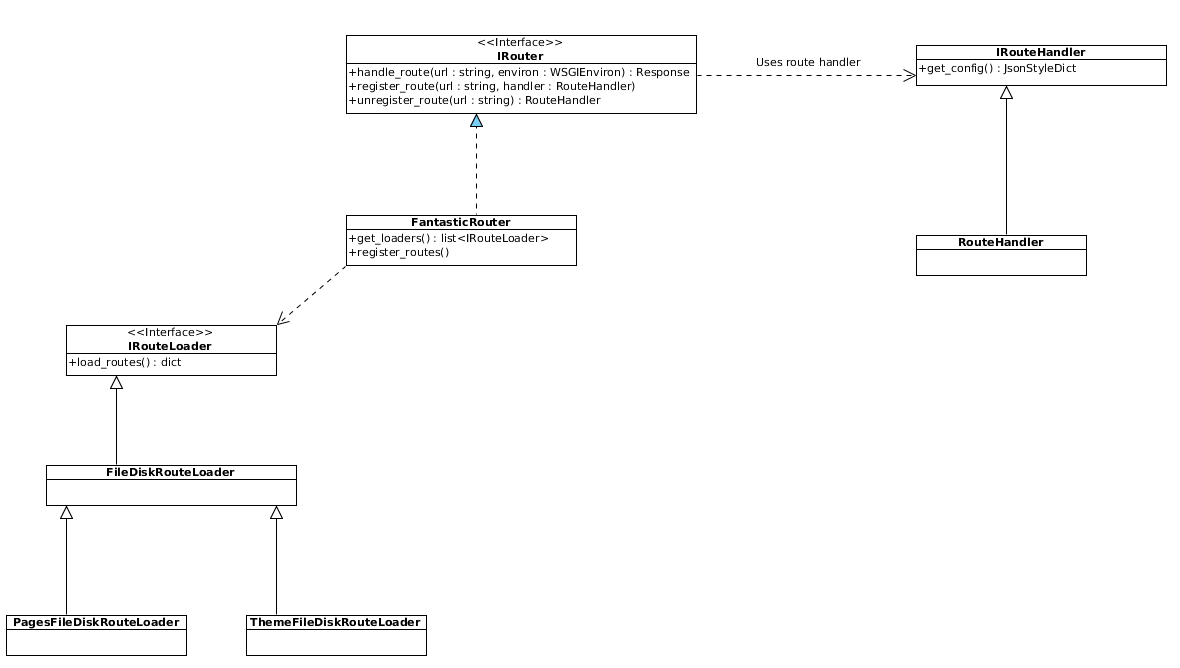
\includegraphics{routing_engine.png}

Fantastico routing engine is design by having extensibility in mind. Below you can find the list of concerns for routing engine:
\begin{enumerate}
\item {} 
Support multiple sources for routes.

\item {} 
Load all available routes.

\item {} 
Select the controller that can handle the request route (if any available).

\end{enumerate}
\index{Router (class in fantastico.routing\_engine.router)}

\begin{fulllineitems}
\phantomsection\label{features/routing_engine:fantastico.routing_engine.router.Router}\pysiglinewithargsret{\strong{class }\code{fantastico.routing\_engine.router.}\bfcode{Router}}{\emph{settings\_facade=\textless{}class `fantastico.settings.SettingsFacade'\textgreater{}}}{}
This class is used for registering all available routes by using all registered loaders.
\index{get\_loaders() (fantastico.routing\_engine.router.Router method)}

\begin{fulllineitems}
\phantomsection\label{features/routing_engine:fantastico.routing_engine.router.Router.get_loaders}\pysiglinewithargsret{\bfcode{get\_loaders}}{}{}
Method used to retrieve all available loaders. If loaders are not currently instantiated they are by these method.
This method also supports multi threaded workers mode of wsgi with really small memory footprint. It uses an internal
lock so that it makes sure available loaders are instantiated only once per wsgi worker.

\end{fulllineitems}

\index{handle\_route() (fantastico.routing\_engine.router.Router method)}

\begin{fulllineitems}
\phantomsection\label{features/routing_engine:fantastico.routing_engine.router.Router.handle_route}\pysiglinewithargsret{\bfcode{handle\_route}}{\emph{url}, \emph{environ}}{}
Method used to identify the given url method handler. It enrich the environ dictionary with a new entry that
holds a controller instance and a function to be executed from that controller.

\end{fulllineitems}

\index{register\_routes() (fantastico.routing\_engine.router.Router method)}

\begin{fulllineitems}
\phantomsection\label{features/routing_engine:fantastico.routing_engine.router.Router.register_routes}\pysiglinewithargsret{\bfcode{register\_routes}}{}{}
Method used to register all routes from all loaders. If the loaders are not yet initialized this method will first
load all available loaders and then it will register all available routes. Also, this method initialize available routes
only once when it is first invoked.

\end{fulllineitems}


\end{fulllineitems}



\subsection{Routes loaders}
\label{features/routing_engine:routes-loaders}
Fantastico routing engine is designed so that routes can be loaded from multiple sources (database, disk locations, and others).
This give huge extensibility so that developers can use Fantastico in various scenarios:
\begin{itemize}
\item {} 
Create a CMS that allows people to create new pages (mapping between page url / controller) is hold in database. Just by
adding a simple loader in which the business logic is encapsulated allows routing engine extension.

\item {} 
Create a blog that loads articles from disk.

\end{itemize}

I am sure you can find other use cases in which you benefit from this extension point.


\subsection{How to write a new route loader}
\label{features/routing_engine:how-to-write-a-new-route-loader}
Before digging in further details see the RouteLoader class documentation below:
\index{RouteLoader (class in fantastico.routing\_engine.routing\_loaders)}

\begin{fulllineitems}
\phantomsection\label{features/routing_engine:fantastico.routing_engine.routing_loaders.RouteLoader}\pysiglinewithargsret{\strong{class }\code{fantastico.routing\_engine.routing\_loaders.}\bfcode{RouteLoader}}{\emph{settings\_facade}}{}
This class provides the contract that must be provided by each concrete implementation. Each route loader is responsible
for implementing its own business logic for loading routes.

\begin{Verbatim}[commandchars=\\\{\}]
\PYG{k}{class} \PYG{n+nc}{DummyRouteLoader}\PYG{p}{(}\PYG{n}{RouteLoader}\PYG{p}{)}\PYG{p}{:}
    \PYG{k}{def} \PYG{n+nf}{\PYGZus{}\PYGZus{}init\PYGZus{}\PYGZus{}}\PYG{p}{(}\PYG{n+nb+bp}{self}\PYG{p}{,} \PYG{n}{settings\PYGZus{}facade}\PYG{o}{=}\PYG{n}{SettingsFacade}\PYG{p}{)}\PYG{p}{:}
        \PYG{n}{self\PYGZus{}settings\PYGZus{}facade} \PYG{o}{=} \PYG{n}{settings\PYGZus{}facade}\PYG{p}{(}\PYG{p}{)}
        
    \PYG{k}{def} \PYG{n+nf}{load\PYGZus{}routes}\PYG{p}{(}\PYG{n+nb+bp}{self}\PYG{p}{)}\PYG{p}{:}
        \PYG{k}{return} \PYG{p}{\PYGZob{}}\PYG{l+s}{\PYGZdq{}}\PYG{l+s}{/index.html}\PYG{l+s}{\PYGZdq{}}\PYG{p}{,} \PYG{l+s}{\PYGZdq{}}\PYG{l+s}{fantastico.plugins.static\PYGZus{}assets.StaticAssetsController.resolve\PYGZus{}text}\PYG{l+s}{\PYGZdq{}}\PYG{p}{,}
                \PYG{l+s}{\PYGZdq{}}\PYG{l+s}{/images/image.png}\PYG{l+s}{\PYGZdq{}}\PYG{p}{,} \PYG{l+s}{\PYGZdq{}}\PYG{l+s}{fantastico.plugins.static\PYGZus{}assets.StaticAssetsController.resolve\PYGZus{}binary}\PYG{l+s}{\PYGZdq{}}\PYG{p}{\PYGZcb{}}
\end{Verbatim}
\index{load\_routes() (fantastico.routing\_engine.routing\_loaders.RouteLoader method)}

\begin{fulllineitems}
\phantomsection\label{features/routing_engine:fantastico.routing_engine.routing_loaders.RouteLoader.load_routes}\pysiglinewithargsret{\bfcode{load\_routes}}{}{}
This method must be overriden by each concrete implementation so that all loaded routes can be handled by
fantastico routing engine middleware.

\end{fulllineitems}


\end{fulllineitems}


As you can, each concrete route loader receives in the constructor settings facade that can be used to access fantastico settings.
In the code example above, DummyRouteLoader maps a list of urls to a controller method that can be used to render it. Keep in
mind that a route loader is a stateless component and it can't in anyway determine the wsgi environment in which it is used. In
addition this design decision also make sure clear separation of concerned is followed.

Once your \textbf{RouteLoader} implementation is ready you must register it into settings profile. The safest bet is to add it into
BaseSettings provider. For more information read {\hyperref[get_started/settings::doc]{\emph{Fantastico settings}}}.


\subsection{Configuring available loaders}
\label{features/routing_engine:configuring-available-loaders}
You can find all available loaders for the framework configured in your settings profile. You can find below a sample
configuration of available loaders:

\begin{Verbatim}[commandchars=\\\{\}]
\PYG{k}{class} \PYG{n+nc}{CustomSettings}\PYG{p}{(}\PYG{n}{BasicSettings}\PYG{p}{)}\PYG{p}{:}
    \PYG{n+nd}{@property}
    \PYG{k}{def} \PYG{n+nf}{routes\PYGZus{}loaders}\PYG{p}{(}\PYG{n+nb+bp}{self}\PYG{p}{)}\PYG{p}{:}
        \PYG{k}{return} \PYG{p}{[}\PYG{l+s}{\PYGZdq{}}\PYG{l+s}{fantastico.routing\PYGZus{}engine.custom\PYGZus{}loader.CustomLoader}\PYG{l+s}{\PYGZdq{}}\PYG{p}{]}
\end{Verbatim}

The above configuration tells \textbf{Fantastico routing engine} that only CustomLoader is a source of routes. If you want to learn
more about multiple configurations please read {\hyperref[get_started/settings::doc]{\emph{Fantastico settings}}}.


\subsection{DummyRouteLoader}
\label{features/routing_engine:dummyrouteloader}\index{DummyRouteLoader (class in fantastico.routing\_engine.dummy\_routeloader)}

\begin{fulllineitems}
\phantomsection\label{features/routing_engine:fantastico.routing_engine.dummy_routeloader.DummyRouteLoader}\pysiglinewithargsret{\strong{class }\code{fantastico.routing\_engine.dummy\_routeloader.}\bfcode{DummyRouteLoader}}{\emph{settings\_facade}}{}
This class represents an example of how to write a route loader. \textbf{DummyRouteLoader} is available in all configurations
and it provides a single route to the routing engine: \emph{/dummy/route/loader/test}. Integration tests rely on this loader
to be configured in each available profile.
\index{display\_test() (fantastico.routing\_engine.dummy\_routeloader.DummyRouteLoader method)}

\begin{fulllineitems}
\phantomsection\label{features/routing_engine:fantastico.routing_engine.dummy_routeloader.DummyRouteLoader.display_test}\pysiglinewithargsret{\bfcode{display\_test}}{\emph{request}}{}
This method handles \textbf{/dummy/route/loader/test route}. It is expected to receive a response with status code 400.
We do this for being able to test rendering and also avoid false positive security scans messages.

\end{fulllineitems}


\end{fulllineitems}



\subsection{Routing middleware}
\label{features/routing_engine:routing-middleware}
\textbf{Fantastico} routing engine is designed as a standalone component. In order to be able to integrate it into Fantastico request
lifecycle (:doc:/features/request\_response.) we need an adapter component.
\index{RoutingMiddleware (class in fantastico.middleware.routing\_middleware)}

\begin{fulllineitems}
\phantomsection\label{features/routing_engine:fantastico.middleware.routing_middleware.RoutingMiddleware}\pysiglinewithargsret{\strong{class }\code{fantastico.middleware.routing\_middleware.}\bfcode{RoutingMiddleware}}{\emph{app}, \emph{router\_cls=\textless{}class `fantastico.routing\_engine.router.Router'\textgreater{}}}{}
Class used to integrate routing engine fantastico component into request / response lifecycle. This middleware is 
responsible for:
\begin{enumerate}
\item {} 
instantiating the router component and make it available to other components / middlewares through WSGI environment.

\item {} 
register all configured fantastico loaders ({\hyperref[features/routing_engine:fantastico.routing_engine.router.Router.get_loaders]{\code{fantastico.routing\_engine.router.Router.get\_loaders()}}}).

\item {} 
register all available routes ({\hyperref[features/routing_engine:fantastico.routing_engine.router.Router.register_routes]{\code{fantastico.routing\_engine.router.Router.register\_routes()}}}).

\item {} 
handle route requests ({\hyperref[features/routing_engine:fantastico.routing_engine.router.Router.handle_route]{\code{fantastico.routing\_engine.router.Router.handle\_route()}}}).

\end{enumerate}

It is important to understand that routing middleware assume a \textbf{WebOb request} available into WSGI environ. Otherwise, 
{\hyperref[features/exceptions:fantastico.exceptions.FantasticoNoRequestError]{\code{fantastico.exceptions.FantasticoNoRequestError}}} will be thrown. You can read more about request middleware 
at {\hyperref[features/request_response::doc]{\emph{Request lifecycle}}}.

\end{fulllineitems}



\chapter{Build status}
\label{index:build-status}
If you want to see the current build status of the project visit \href{http://jenkins.scrum-expert.ro:8080/job/fantastico-framework/badge/icon/}{Build status}.


\chapter{License}
\label{index:license}
Copyright 2013 Cosnita Radu Viorel

Permission is hereby granted, free of charge, to any person obtaining a copy of this software and associated
documentation files (the ``Software''), to deal in the Software without restriction, including without limitation
the rights to use, copy, modify, merge, publish, distribute, sublicense, and/or sell copies of the Software,
and to permit persons to whom the Software is furnished to do so, subject to the following conditions:

The above copyright notice and this permission notice shall be included in all copies or substantial portions of the Software.

THE SOFTWARE IS PROVIDED ``AS IS'', WITHOUT WARRANTY OF ANY KIND, EXPRESS OR IMPLIED, INCLUDING BUT NOT LIMITED TO THE
WARRANTIES OF MERCHANTABILITY, FITNESS FOR A PARTICULAR PURPOSE AND NONINFRINGEMENT. IN NO EVENT SHALL THE AUTHORS OR
COPYRIGHT HOLDERS BE LIABLE FOR ANY CLAIM, DAMAGES OR OTHER LIABILITY, WHETHER IN AN ACTION OF CONTRACT, TORT OR OTHERWISE,
ARISING FROM, OUT OF OR IN CONNECTION WITH THE SOFTWARE OR THE USE OR OTHER DEALINGS IN THE SOFTWARE.



\renewcommand{\indexname}{Index}
\printindex
\end{document}
